\documentclass[12pt,a4paper]{article}

\input{../../preamble_files/packages}
\input{../../preamble_files/scriptr}
\input{../../preamble_files/siunits}
\input{../../preamble_files/vectors}
\input{../../preamble_files/figures}
\input{../../preamble_files/references}
\input{../../preamble_files/empheq}

\pagestyle{fancy}
\lhead{Richard Whitehill}
\chead{PHYS 631 -- HW G}
\rhead{02/15/22}
\cfoot{\thepage \hspace{1pt} of \pageref{LastPage}}

\newcommand{\prob}[2]{\textbf{#1)} #2}

\setlength{\parskip}{\baselineskip}
\setlength{\parindent}{0pt}

\begin{document}

\prob{2.33}{Consider an infinite chain of point charges, $\pm q$ (with alternating signs), strung out along the $x$ axis, each a distance $a$ from its nearest neighbors. Find the work per particle required to assemble this system.}

\bef
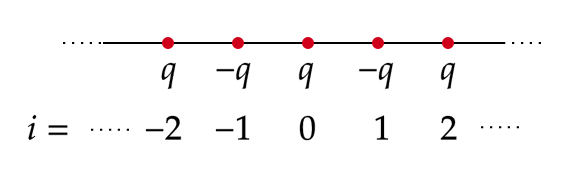
\includegraphics[scale=0.5]{fig1.png}
\eef

The work to assemble a point charge distribution is given as
\begin{align*}
W = \frac{1}{2}\sum_{i}q_i\qty(\sum_{j \not= i} \frac{1}{4\pi\epsilon_0}\frac{q_j}{\scriptr_{ij}})
\end{align*}
For this distribution then, we have
\begin{align*}
W = \frac{1}{2}\sum_{i}(-q)^{i}\qty(\sum_{j \not= i} \frac{1}{4\pi\epsilon_0}\frac{(-q)^{j}}{|i-j|a}) = \frac{1}{4\pi\epsilon_0}\frac{q}{a}\sum_{i} (-1)^{i}\qty(\frac{(-1)^{j}}{|i-j|})
\end{align*}
For simplicity, if we consider $i = 0$, then
\begin{align*}
\sum_{j \not= 0} \frac{(-1)^{j}}{|j|} = \sum_{j=-\infty}^{-1} \frac{(-1)^{j}}{-j} + \sum_{j=1}^{\infty} \frac{(-1)^{j}}{j}
\end{align*}
In the first series, if we let $j \rightarrow -j$, then
\begin{align*}
\sum_{j \not= 0} \frac{(-1)^{j}}{|j|} = 2\sum_{j=1}^{\infty} \frac{(-1)^j}{j} = -2\ln{2}
\end{align*}
The sum here is the alternating harmonic series, which has a well known result and can be found online. Or alternatively, one can infer the final result by looking at the Taylor series expansion of $\ln(x+1)$.

Note that this result is for $i = 0$ corresponding to a charge $+q$. Since the problem is invariant under translations by $\pm a$, we can infer the result for any $i$.
\begin{align*}
\sum_{j \not= i} \frac{(-1)^{j}}{|i-j|} = 2(-1)^{i+1}\ln{2}
\end{align*}
Thus,
\begin{align*}
W = \sum_{i} -\frac{q^2}{4\pi\epsilon_0a}\ln{2}
\end{align*}
The work done here is obviously infinite, but the average work done per particle is just the summand (if that is even a word!). That is
\begin{eqbox}
\left<W\right> = -\frac{q^2}{4\pi\epsilon_0a}\ln{2}
\end{eqbox}


\prob{2.38}{A metal sphere of radius $R$, carrying charge $q$, is surrounded by a thick concentric metal shell (inner radius $a$, outer radius $b$, as in Fig. 2.48). The shell carries no net charge.}

\bef
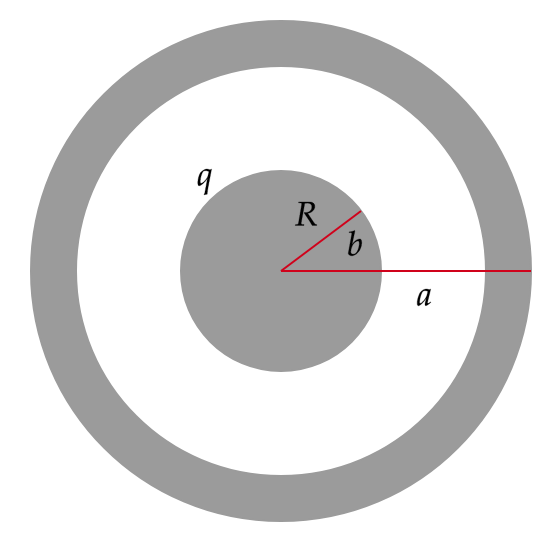
\includegraphics[scale=0.5]{fig2.png}
\eef

(a) Find the surface charge density $\sigma$ at $R$, at $a$, and at $b$.

We can read off the surface charge densities by thinking about induced charges and the surface areas on which they are induced. Thus, we see that
\begin{eqbox}
\sigma_R = \frac{q}{4\pi R^2} \quad \sigma_a = \frac{-q}{4\pi a^2} \quad \sigma_a = \frac{q}{4\pi b^2}
\end{eqbox}

(b) Find the potential at the center, using infinity as the reference point.

We can find the potential using
\begin{align*}
V(0) = -\int_{0}^{\infty} E(r) \dd{r}
\end{align*}
We find the electric field at each $r$ using Gauss's law
\begin{align*}
V(0) = -\qty[\int_{0}^{R} 0\dd{r} + \int_{R}^{a} \frac{1}{4\pi\epsilon_0}\frac{q}{r^2}\dd{r} + \int_{a}^{b} 0 \dd{r} + \int_{b}^{\infty} \frac{1}{4\pi\epsilon_0}\frac{q}{r^2} \dd{r}]
\end{align*}
\begin{eqbox}
V(0) = \frac{q}{4\pi\epsilon_0}\qty(\frac{1}{a} - \frac{1}{R} - \frac{1}{b})
\end{eqbox}

(c) Now the outer surface is touched to a grounding wire, which drains off charge and lowers its potential to zero (same as at infinity). How do your answers to (a) and (b) change?

For part (a) $\sigma_{R,b}$ should remain the same while $\sigma_a = 0$ since all charge on the outer surface is drained off. 

In part (b) the electric field outside of the second volume is zero, since the enclosed charge is zero. Thus, we are left only with $V(0) = q/(4\pi\epsilon_0)(1/a-1/R)$.


\end{document}
